\documentclass[10pt]{article}
\usepackage{amsmath, amssymb}
%\usepackage[pdftex]{graphicx}
\usepackage{graphicx}

\title{Performance of Thyra Adapters in Anasazi}
\author{Thornquist, H. K. and Baker, C. G.}
%\date{}

\begin{document}
\maketitle

\section{Introduction}

Anasazi is a Trilinos package for solving large-scale eigenvalue problems. In order to
achieve as much flexibility as possible, the components of the package are templated
according to scalar type and linear algebra objects (multivectors and operators). The
functionality of these objects are accessed via traits classes, specialized on the
template classes. Therefore, to make use of a particular linear algebra library for the
underlying computation, the user needs only to implement specializations of these traits
classes for the particular linear algebra objects. This creates a sort of wrapper around
the functionality, without requiring the user to modify the inheritance heirarchy of the
classes.

Thyra is a Trilinos package which defines a set of interfaces designed to ease
interoperability of different numerical packages. Filling out specializations of the
Anasazi traits classes allows any underlying linear algebra to be used with Anasazi.
However, designing a linear algebra library in the Thyra framework allows this library to
be used with any numerical software that recognizes Thyra. 

With this in mind, Anasazi provides an adapter (via a traits class specialization) to the
Thyra interfaces, to ease the interoperability of Anasazi with other packages. The goal of
this report is to examine the performance overhead of using this adapter. The purpose of
this is to document any such overhead, as users may be curious about the cost of using
the adapter. Another goal is to discover inefficiencies in the adapter to allow their
remedy.

\section{Methodology}

It is expected that there will be a small amount of overhead resulting from the use of the
Anasazi adapters to Thyra. This overhead should be constant-time, and therefore should
diminish in effect as the size of the problem increases. The study will be the solution of
a general sparse eigenvalue problem.  The overhead will be analyzed by three measures:
total time to solve the problem, time spent manipulating multivectors, and time spent
applying linear operators. Two eigensolvers will be analysed: LOBPCG and Block Davidson.
Block Davidson performs much more multivector manipulation per operator application than
does LOBPCG, and therefore weights those computatations heavier in the total time.

Recall that there are two major players in action during a call to Anasazi: the underlying
linear algebra library and the adapter used to interface this linear algebra library. The
analysis of overhead will be made by comparing two different linear algebra libraries and
two different adapters. The tests will be perfomed for the following scenarios:
\begin{itemize}
\item Epetra\_MultiVector,Epetra\_Op via Epetra adapter
\item Thyra\_MultiVector,Epetra\_Op  via Thyra adapter 
\item Epetra\_MultiVector,Epetra\_Op via Thyra adapter and Epetra-Thyra wrappers
\end{itemize}

The input for each test was from the test class \verb!ModeLaplace1DQ1!, available in the
\verb!anasazi/util! directory in the Trilinos source tree. This is a generalized
eigenvalue problem. Both solvers were limited to a fixed number ($50$) of iterations. The
results were checked to make sure that all three scenarios (Epetra, Thyra, and
Thyra-Epetra) performed similarly.

The three scenarios will be tested in serial and in parallel, for problem sizes of $1e2$,
$1e3$, $1e4$, $1e5$, and $1e6$. On paunchy and sophie, the reported times are the average
of three tests. On qed, the reported times originate from a single run. The times will be
computed on the following platforms:
\begin{itemize}
\item sophie: serial and mpi(2)
\item paunchy: serial, mpi(2), and mpi(4)
\item qed: mpi(2), mpi(4), mpi(8), mpi(16), mpi(32), mpi(64)
\end{itemize}

These platforms are described in the appendix.

\section{Performance}

%-----------------------------------------------------------------------------
%--- Paunchy tests -----------------------------------------------------------
%-----------------------------------------------------------------------------
\subsection{Paunchy}

Paunchy is an SMP Sun machine with 4 processors. We tested Paunchy in three scenarios:
serial, 1 processor MPI and 2 processor MPI. Figure~\ref{fig:Paunchy} shows the results of
the testing. Each cluster of lines represent a choice of platform (serial or mpi), denoted
by the x-axis label. The datapoints inside a cluster show problems of the following sizes
(from left to right, in the cluster): $n=1e2$, $n=1e3$, $n=1e4$, $n=1e5$, $n=1e6$. 

\begin{figure}[htp]
\begin{tabular}{cc}
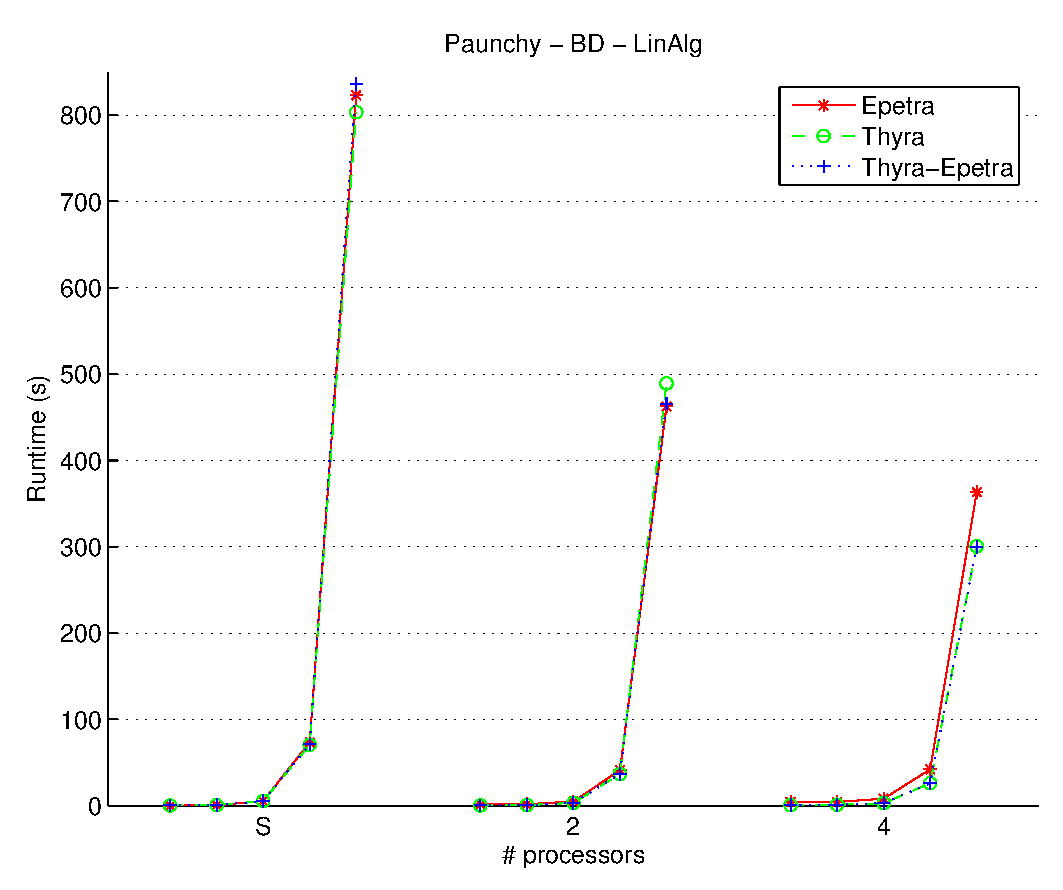
\includegraphics[width=2.50in]{results/paunchy/Paunchy-BD-LinAlg_ln.eps} &
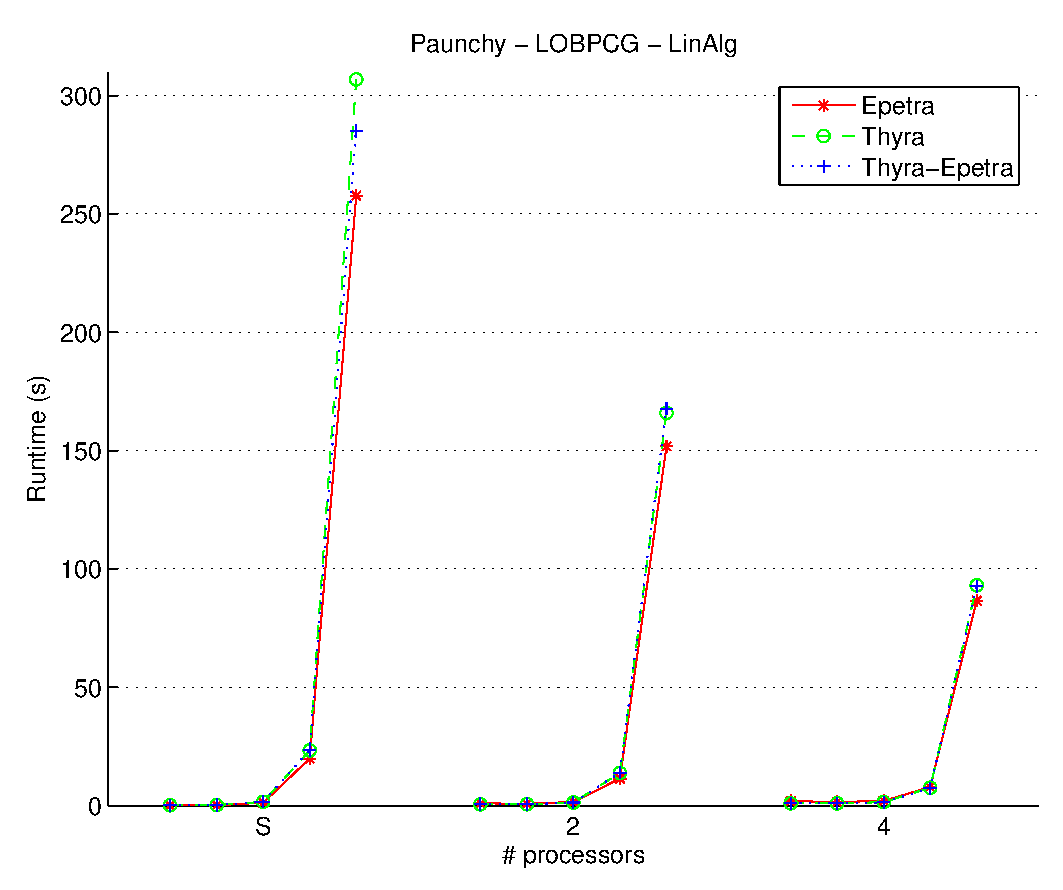
\includegraphics[width=2.50in]{results/paunchy/Paunchy-LOBPCG-LinAlg_ln.eps} \\
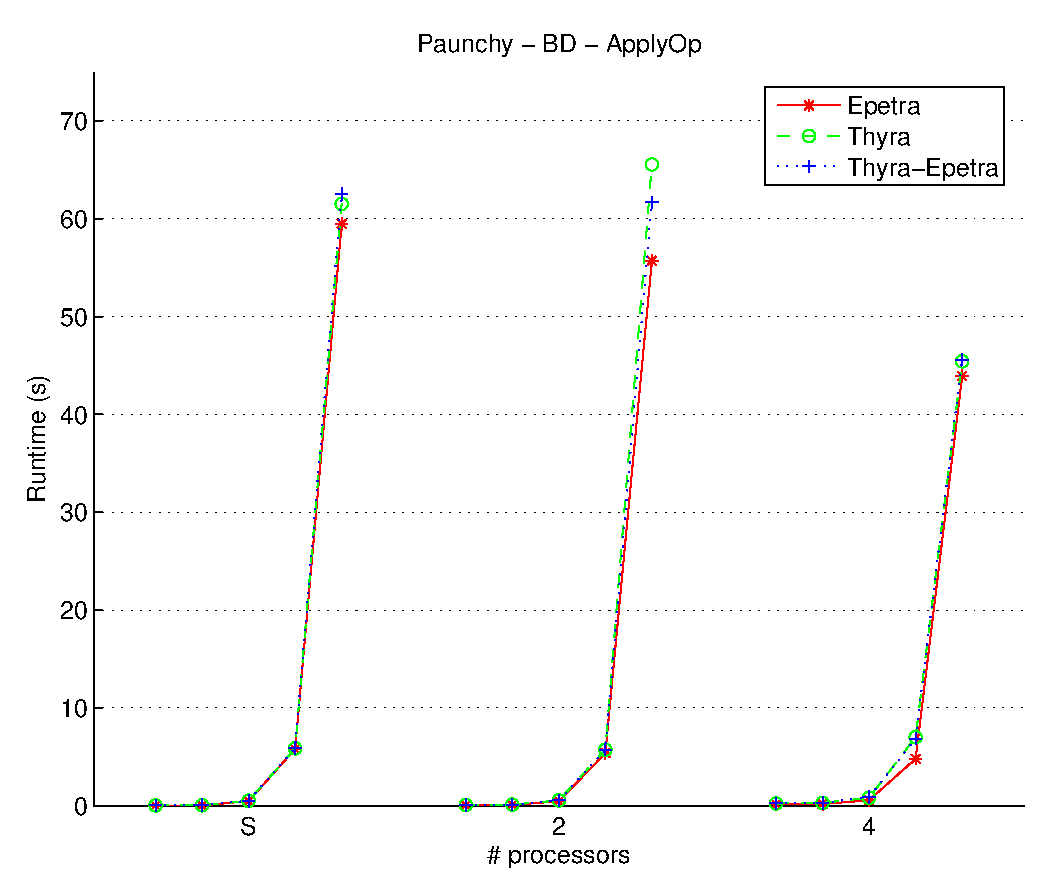
\includegraphics[width=2.50in]{results/paunchy/Paunchy-BD-ApplyOp_ln.eps} &
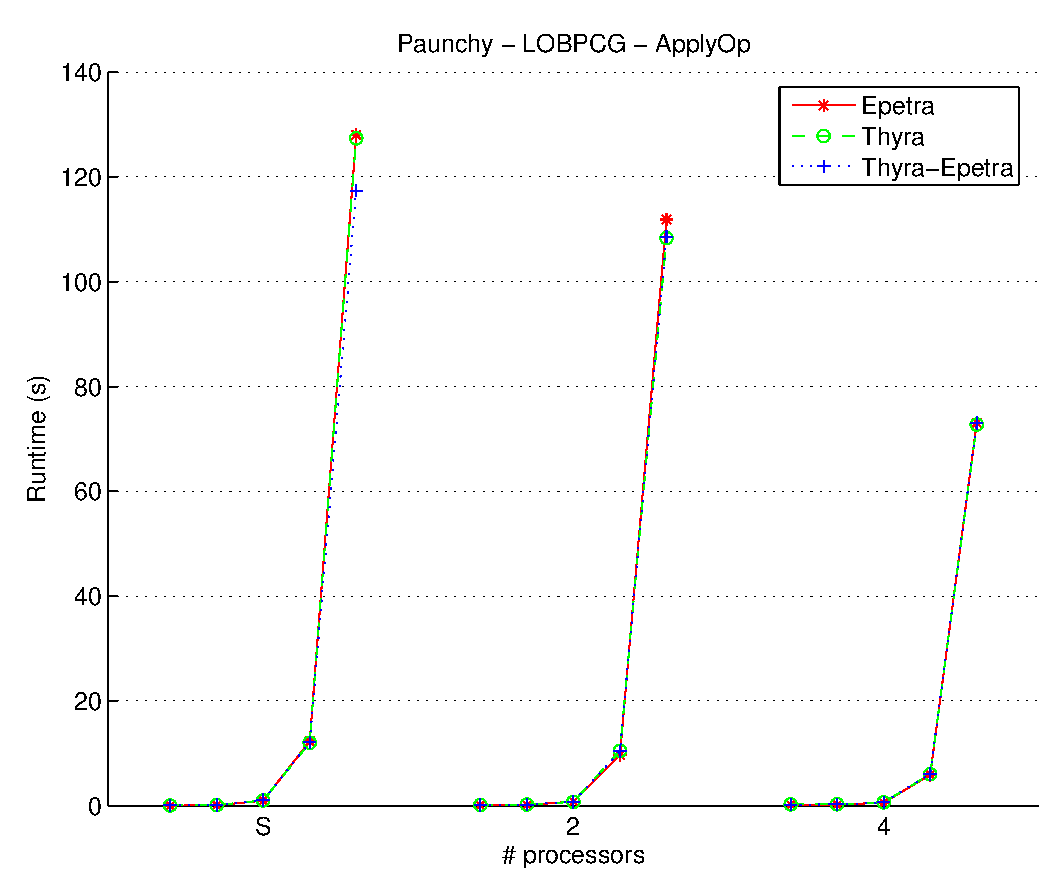
\includegraphics[width=2.50in]{results/paunchy/Paunchy-LOBPCG-ApplyOp_ln.eps} \\
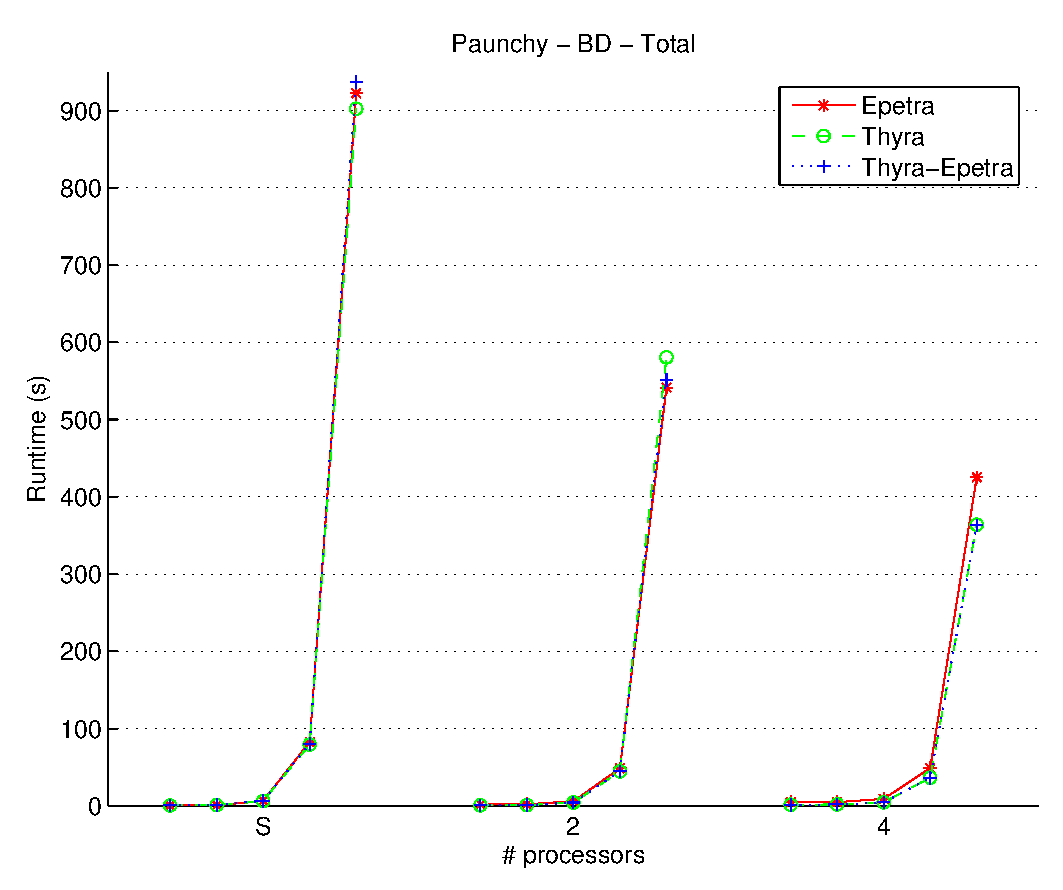
\includegraphics[width=2.50in]{results/paunchy/Paunchy-BD-Total_ln.eps} &
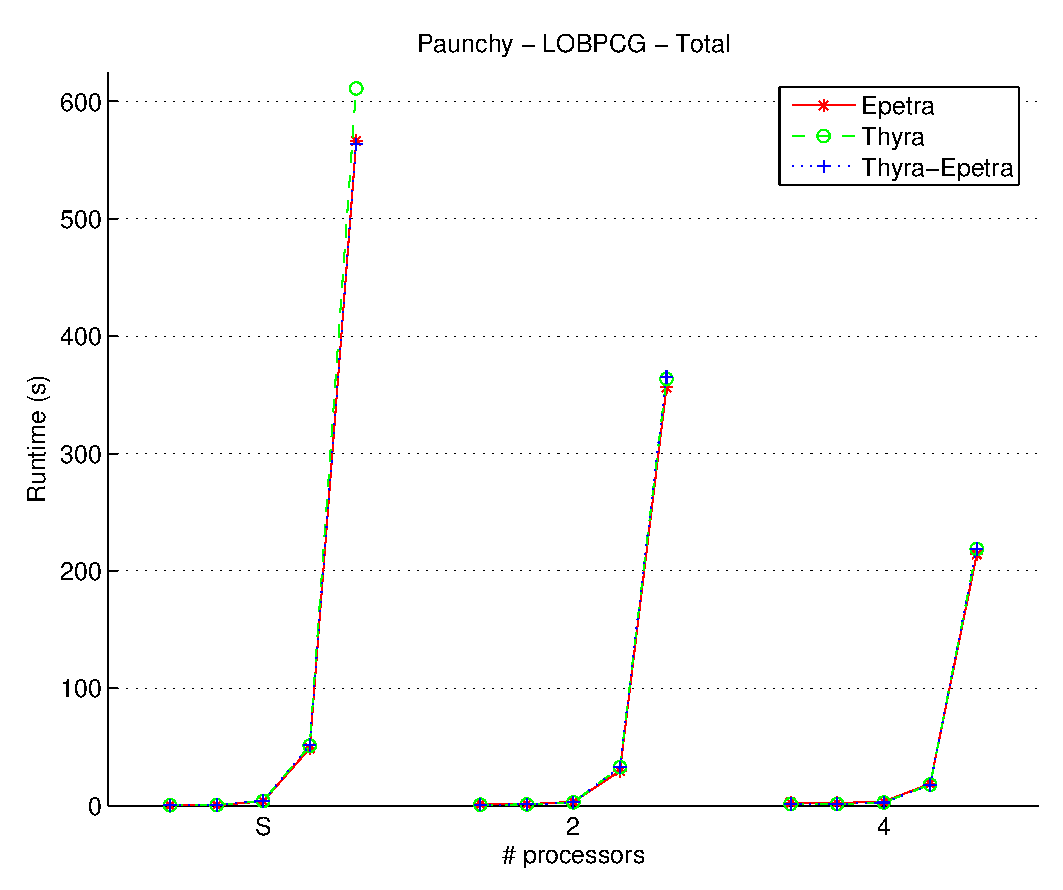
\includegraphics[width=2.50in]{results/paunchy/Paunchy-LOBPCG-Total_ln.eps} 
\end{tabular}
\caption{Performance of Block Davidson and LOBPCG on Paunchy.}
\label{fig:Paunchy}
\end{figure}

%-----------------------------------------------------------------------------
%--- Sophie tests ------------------------------------------------------------
%-----------------------------------------------------------------------------
\subsection{Sophie}

Sophie is a PowerMac G5 with 2 processors. We tested Sophie in two scenarios: serial 
and 2 processor MPI. Figure~\ref{fig:Sophie} shows the results of
the testing. Each cluster of lines represent a choice of platform (serial or mpi), denoted
by the x-axis label. The datapoints inside a cluster show problems of the following sizes
(from left to right, in the cluster): $n=1e2$, $n=1e3$, $n=1e4$, $n=1e5$, $n=1e6$.


\begin{figure}[htp]
\begin{tabular}{cc}
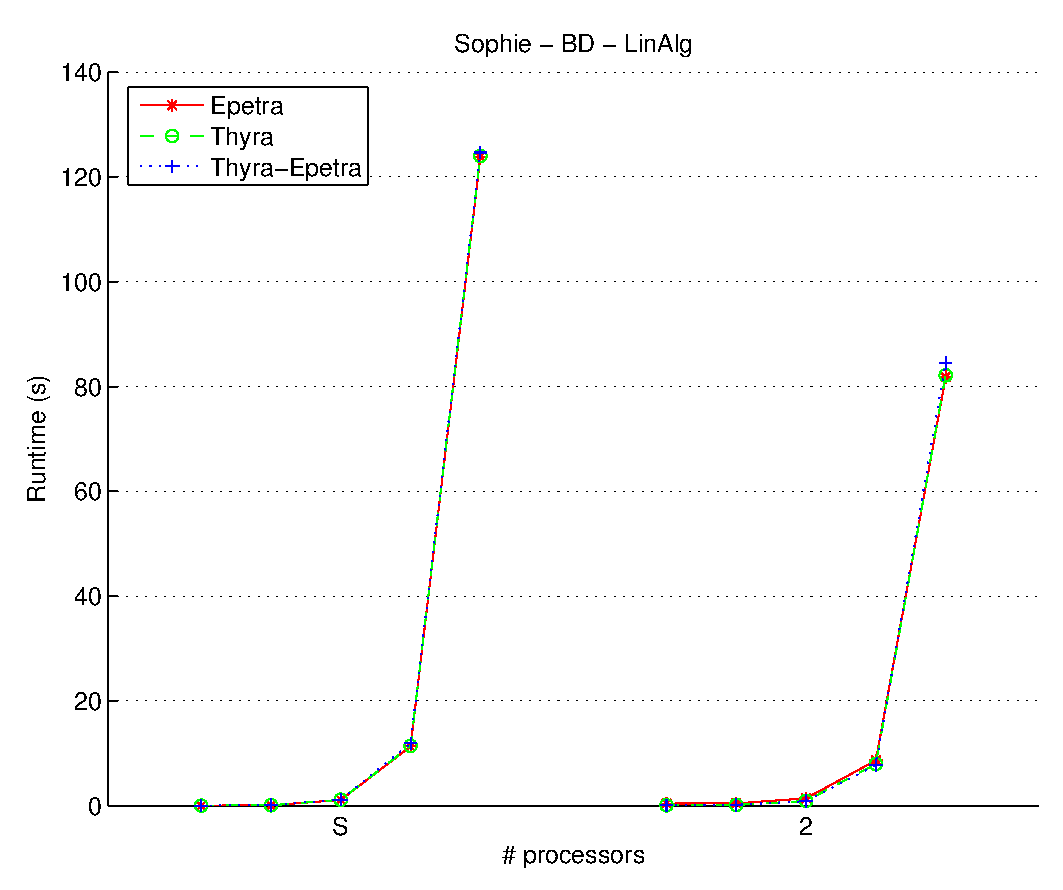
\includegraphics[width=2.50in]{results/sophie/Sophie-BD-LinAlg_ln.eps} &
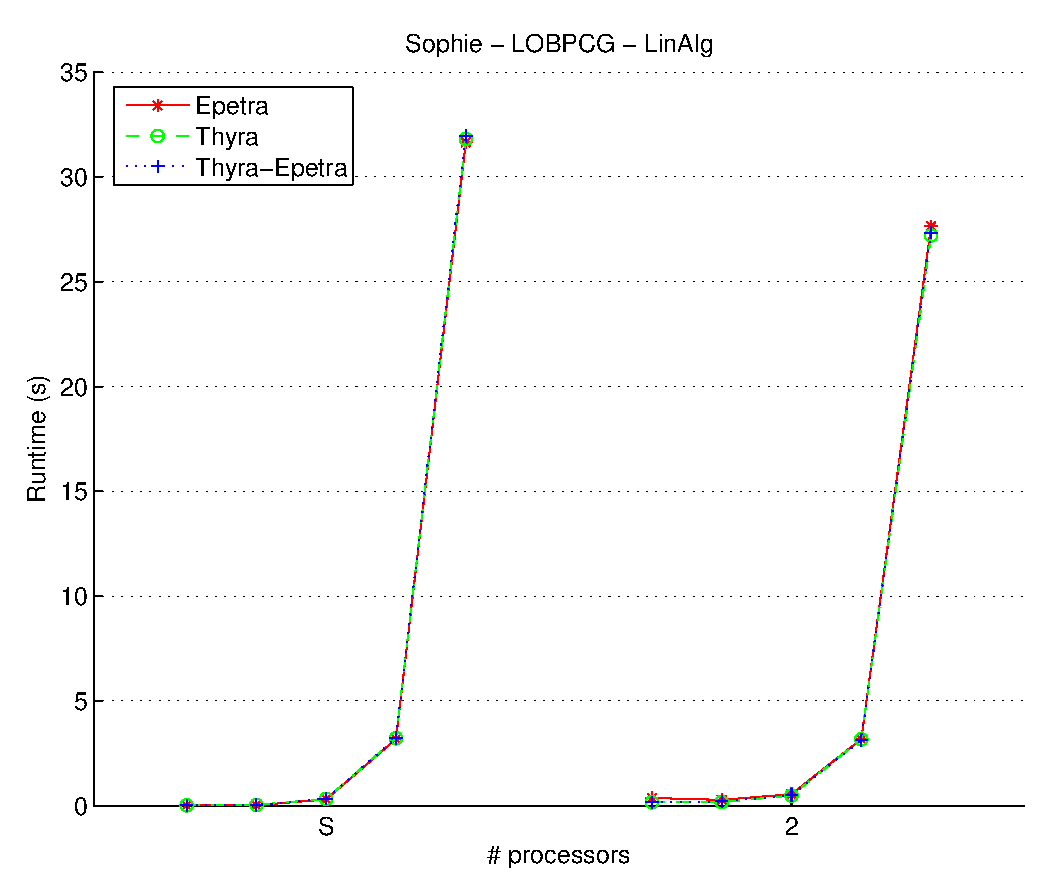
\includegraphics[width=2.50in]{results/sophie/Sophie-LOBPCG-LinAlg_ln.eps} \\
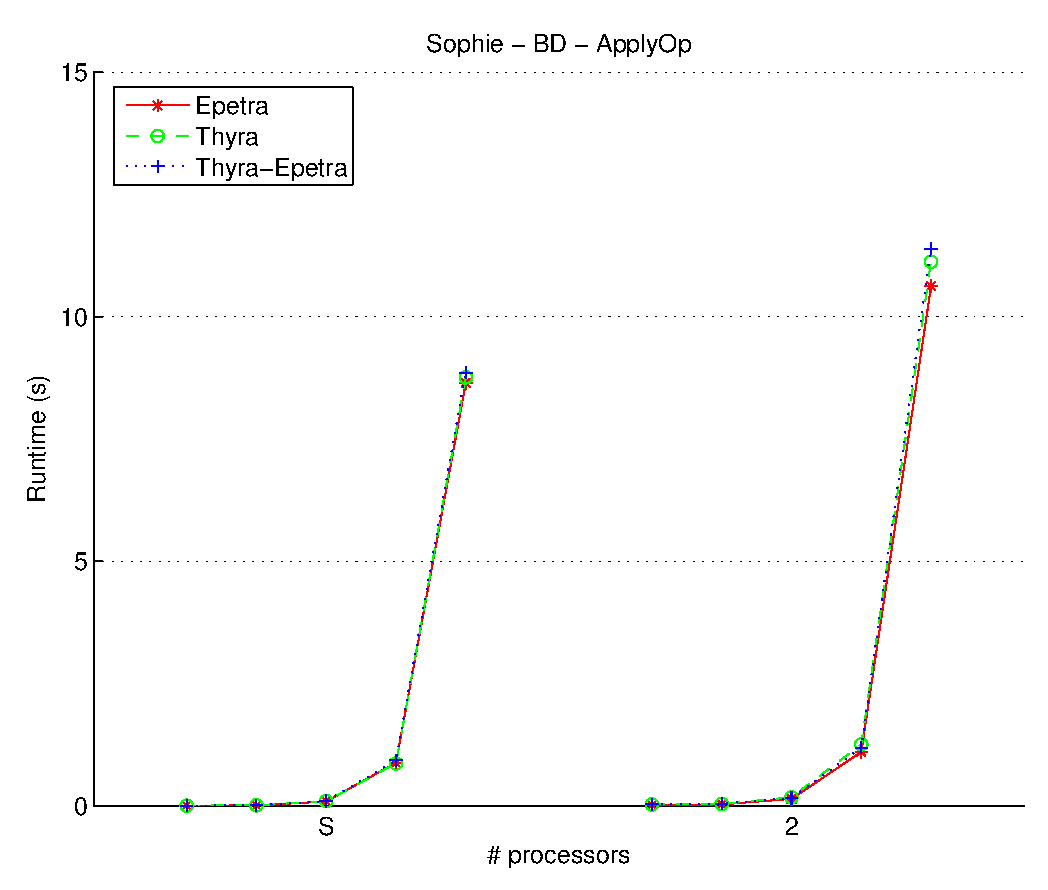
\includegraphics[width=2.50in]{results/sophie/Sophie-BD-ApplyOp_ln.eps} &
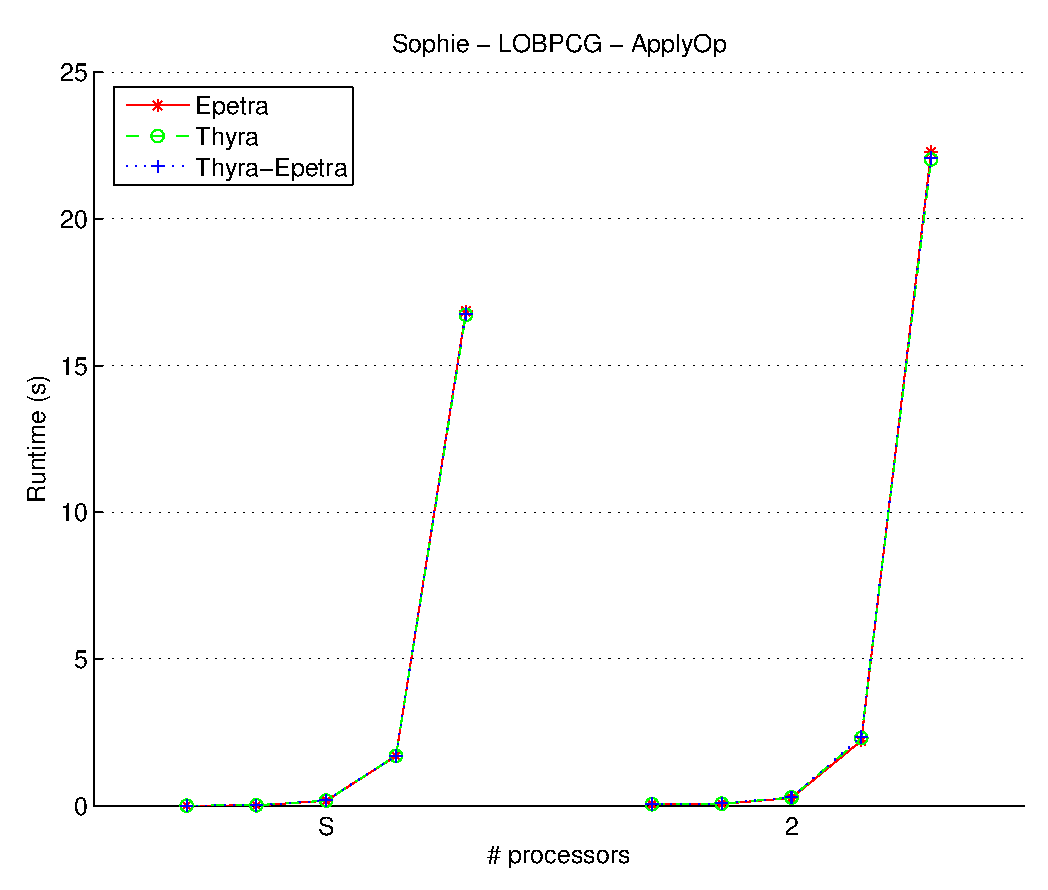
\includegraphics[width=2.50in]{results/sophie/Sophie-LOBPCG-ApplyOp_ln.eps} \\
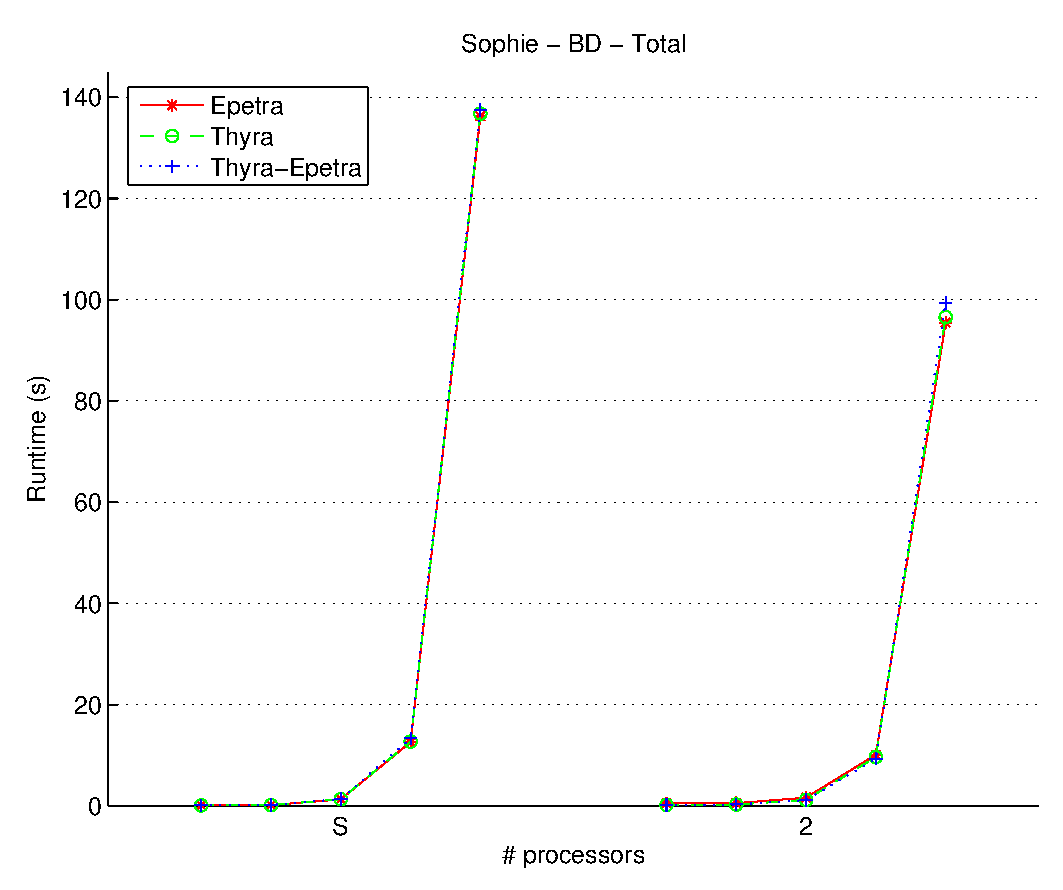
\includegraphics[width=2.50in]{results/sophie/Sophie-BD-Total_ln.eps} &
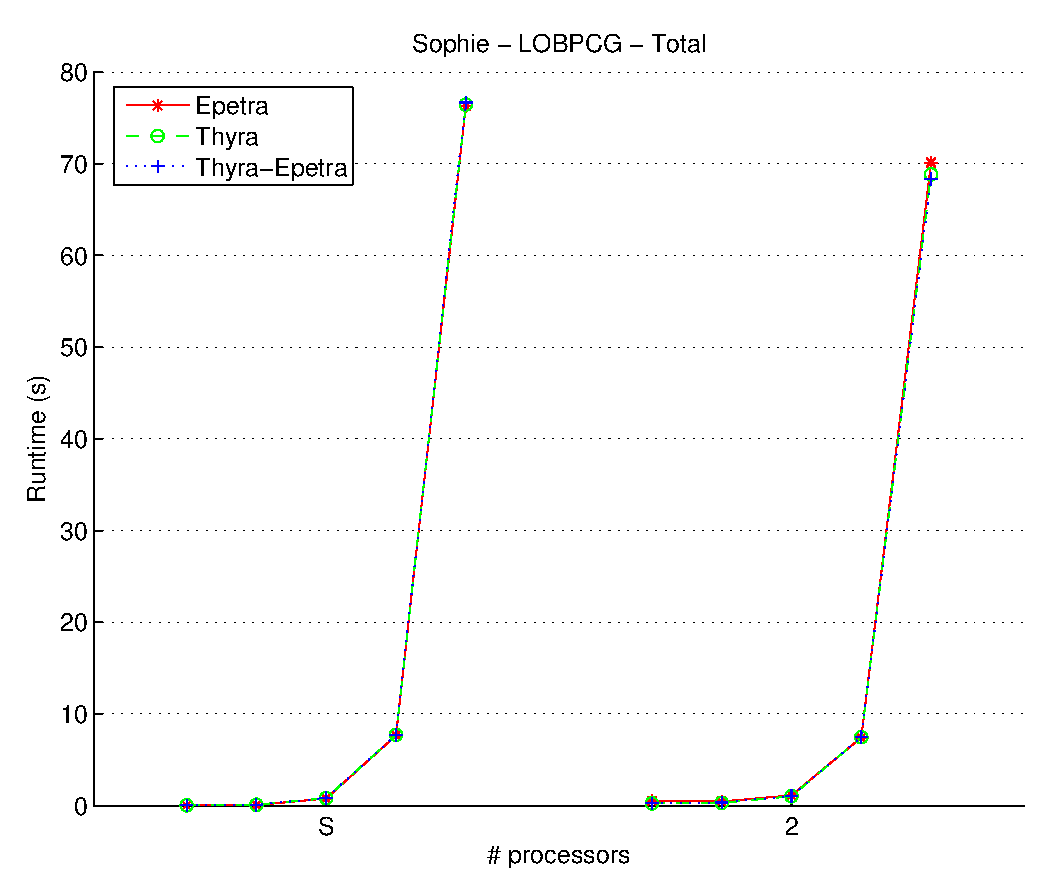
\includegraphics[width=2.50in]{results/sophie/Sophie-LOBPCG-Total_ln.eps} 
\end{tabular}
\caption{Performance of Block Davidson and LOBPCG on Sophie.}
\label{fig:Sophie}
\end{figure}


%-----------------------------------------------------------------------------
%--- QED tests ------------------------------------------------------------
%-----------------------------------------------------------------------------
\subsection{QED}

QED is a linux cluster with 32 nodes of 2 processors each. We tested QED in five
scenarios: 2 processors, 4 processors, 8 processors, 16 processors, 32
processors and 64 processors. Figure~\ref{fig:Sophie} shows the results of
the testing. Each cluster of lines represent a choice of platform (serial or mpi), denoted
by the x-axis label. The datapoints inside a cluster show problems of the following sizes
(from left to right, in the cluster): $n=1e2$, $n=1e3$, $n=1e4$, $n=1e5$, $n=1e6$.

\begin{figure}[htp]
\begin{tabular}{cc}
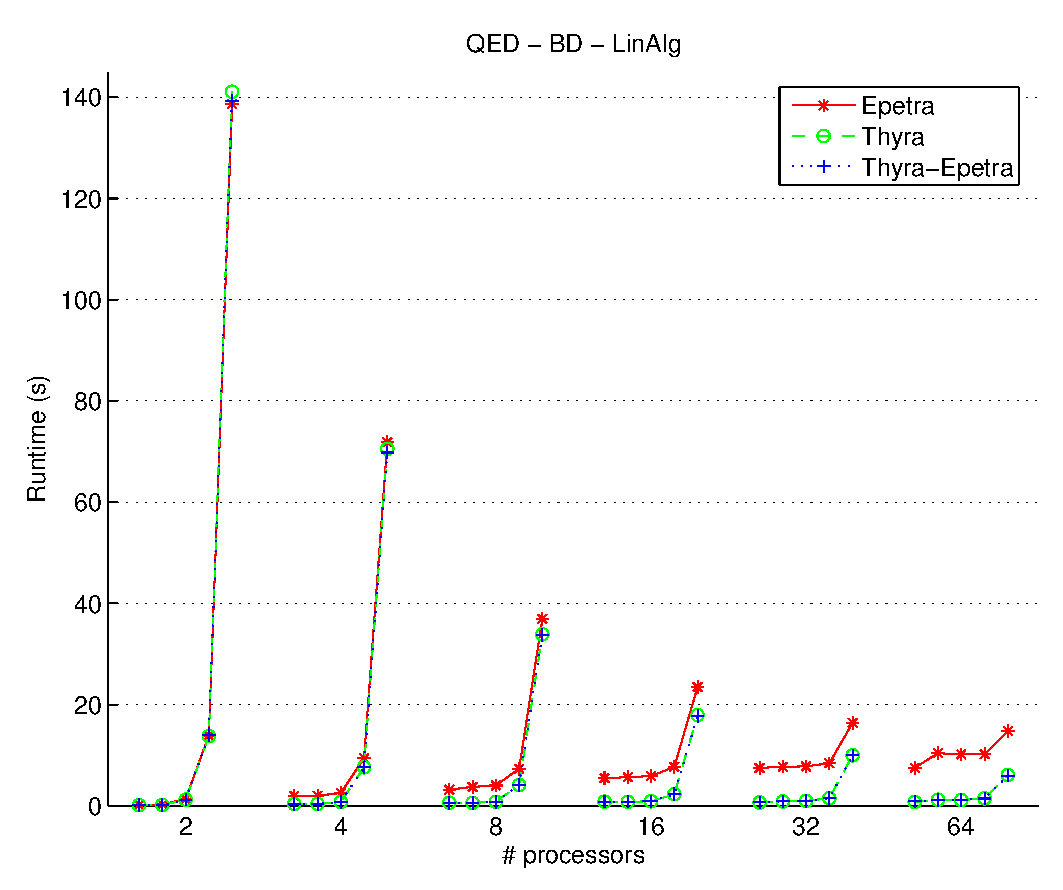
\includegraphics[width=2.50in]{results/qed/QED-BD-LinAlg_ln.eps} &
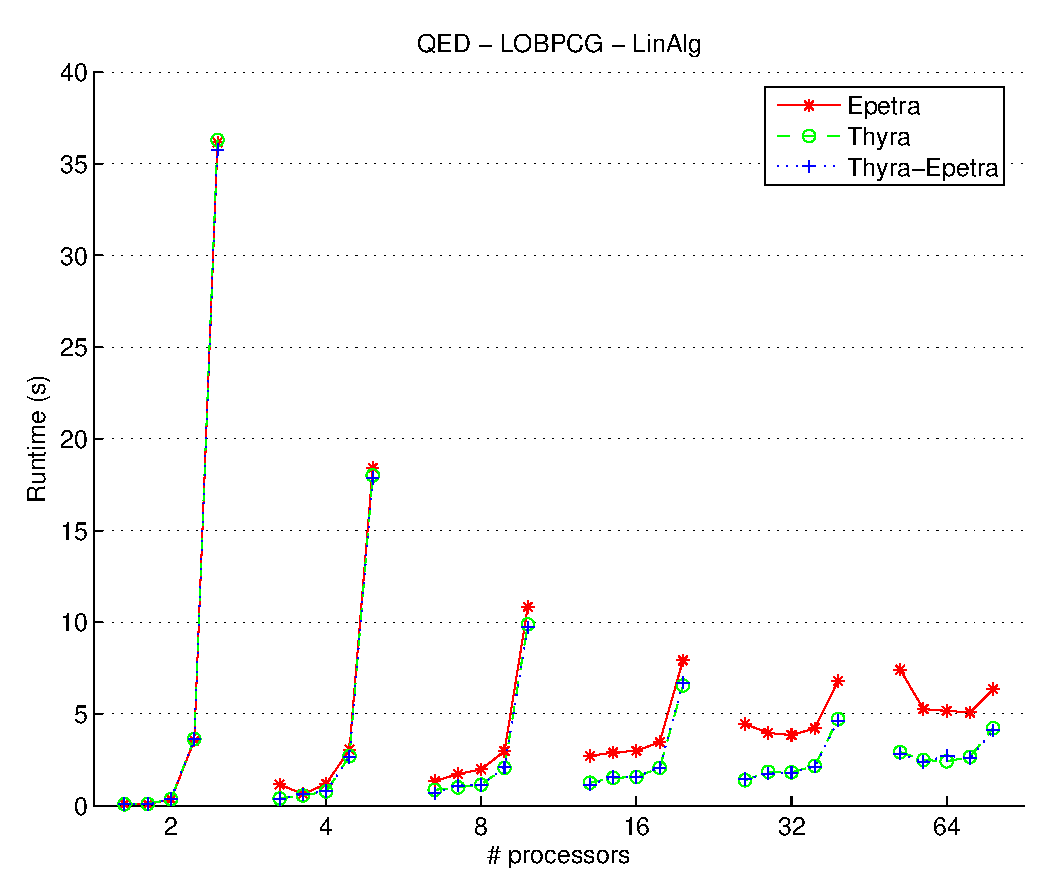
\includegraphics[width=2.50in]{results/qed/QED-LOBPCG-LinAlg_ln.eps} \\
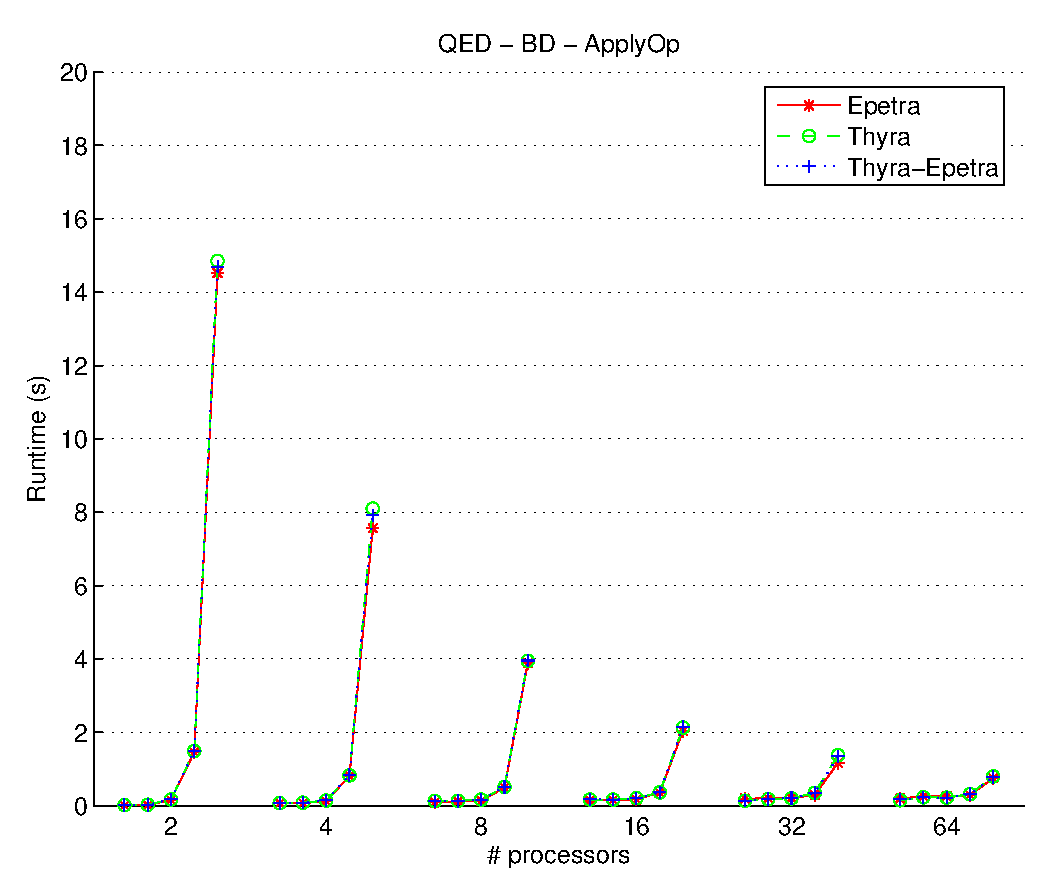
\includegraphics[width=2.50in]{results/qed/QED-BD-ApplyOp_ln.eps} &
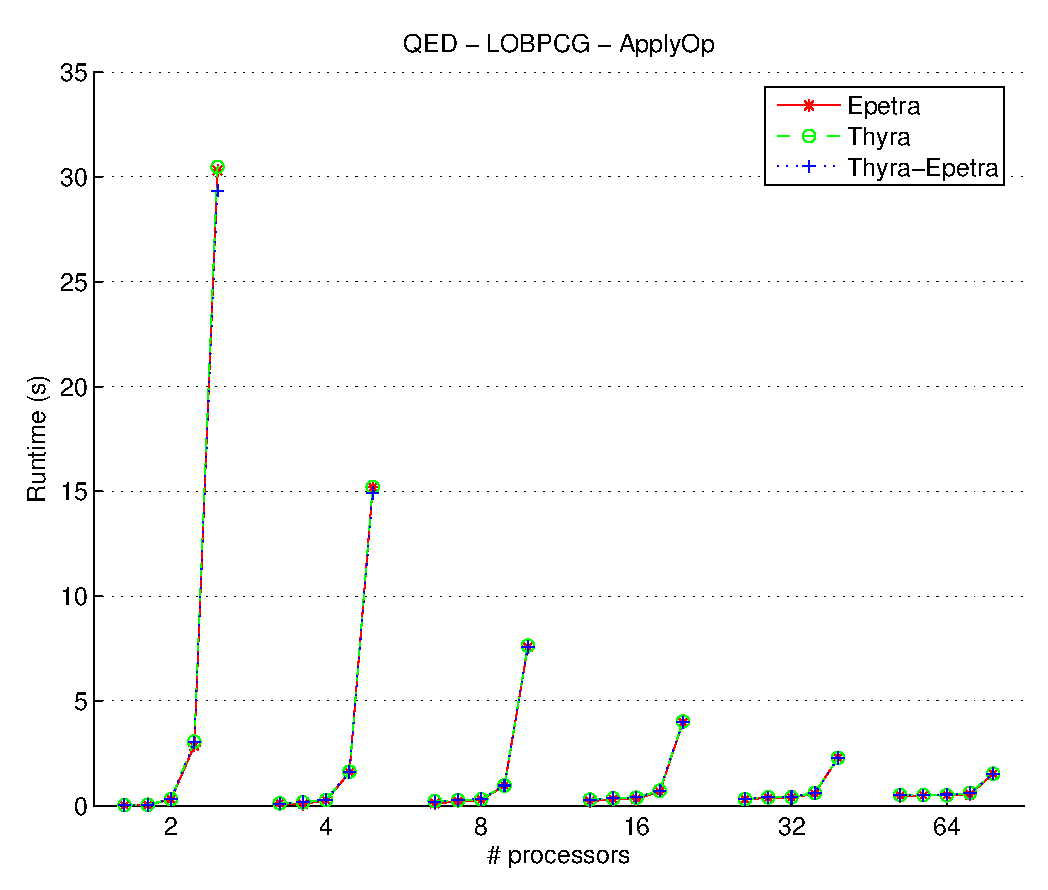
\includegraphics[width=2.50in]{results/qed/QED-LOBPCG-ApplyOp_ln.eps} \\
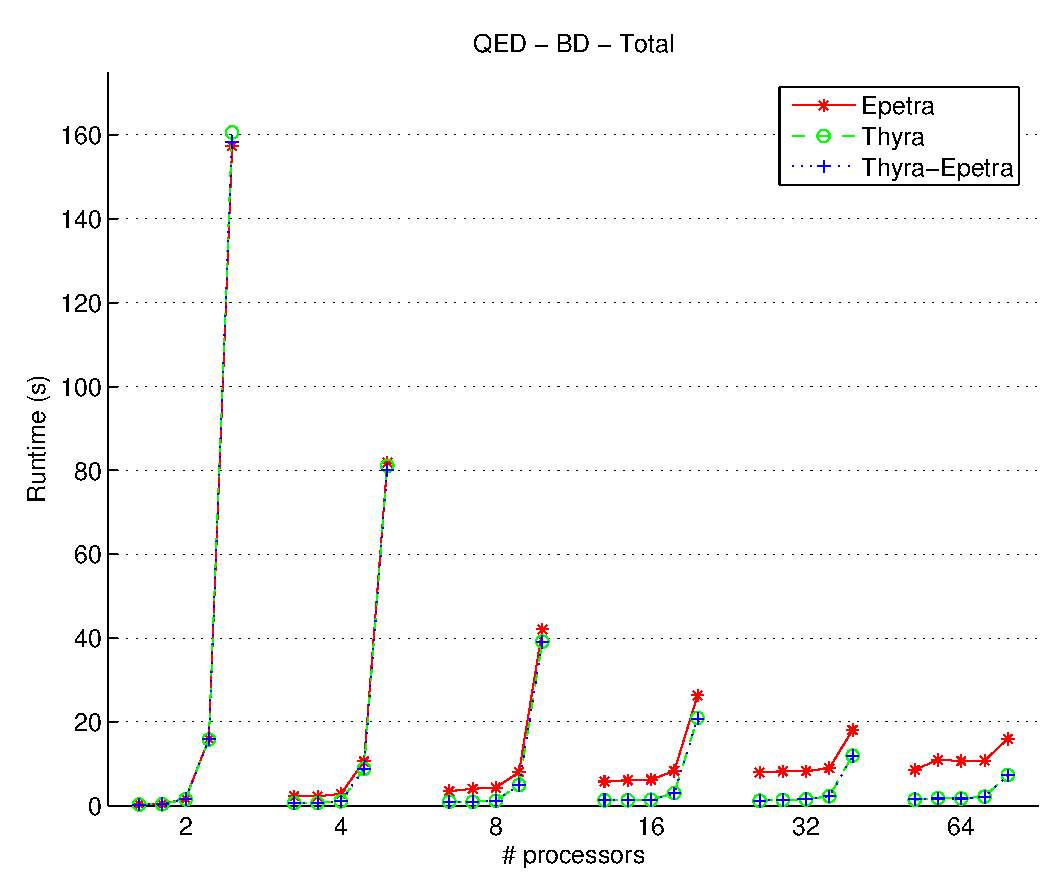
\includegraphics[width=2.50in]{results/qed/QED-BD-Total_ln.eps} &
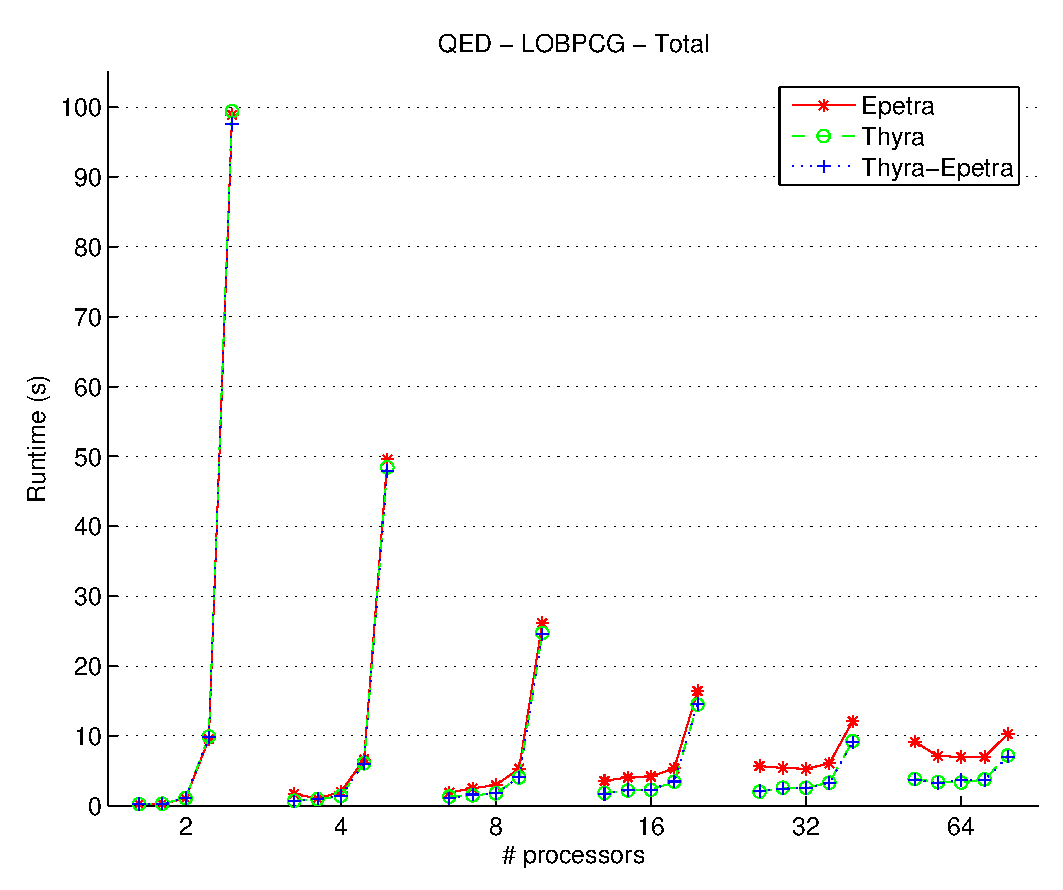
\includegraphics[width=2.50in]{results/qed/QED-LOBPCG-Total_ln.eps} 
\end{tabular}
\caption{Performance of Block Davidson and LOBPCG on QED.}
\label{fig:QED}
\end{figure}


\section{Conclusion}

A quick glance at the figures shows that there are little penalties associated with the
use of the Thyra adapters. In fact, because the Thyra adapters to Epetra multivectors are
``fake'' adapters (in the sense that they do not wrap the Epetra multivector
functionality, but only the data), the performance of the Thyra implementation can surpass
that of the Epetra implementation. This trend is noticeable as the number of processors
increases.

In conclusion, we have documented the performance of three impelementation of Anasazi.
The results indicate that there is little penalty associated with choosing any particular
implementation. Furthermore, the results do not indicate any obvious problems with the
implementation of the adapters.

%%%%%%%%%%%%%%%%%%%%%%%%%%%%%%%%%%%%%%%%%%%%%%%%%%%%%%%%%%%%%%%%%%%%%%%%%%%%%%%%%%%%%%%%%%
%%%%%%%%%%%%%%%%%%%%%%%%%%%%%%%%%%%%%%%%%%%%%%%%%%%%%%%%%%%%%%%%%%%%%%%%%%%%%%%%%%%%%%%%%%
%%%%%%%%%%%%%%%%%%%%%%%%%%%%%%%%%%%%%%%%%%%%%%%%%%%%%%%%%%%%%%%%%%%%%%%%%%%%%%%%%%%%%%%%%%
%%%%%%%%%%%%%%%%%%%%%%%%%%%%%%%%%%%%%%%%%%%%%%%%%%%%%%%%%%%%%%%%%%%%%%%%%%%%%%%%%%%%%%%%%%
\appendix
\section{Platforms}

Paunchy is an SMP Solaris machine with the following statistics:
\begin{verbatim}
paunchy$ uname -a
SunOS paunchy 5.8 Generic_108528-29 sun4u sparc SUNW,Ultra-80

paunchy$ prtdiag
System Configuration:  Sun Microsystems  sun4u \
   Sun Enterprise 420R (4 X UltraSPARC-II 450MHz)
System clock frequency: 113 MHz
Memory size: 4096 Megabytes

========================= CPUs =========================

                    Run   Ecache   CPU    CPU
Brd  CPU   Module   MHz     MB    Impl.   Mask
---  ---  -------  -----  ------  ------  ----
 0     0     0      450     4.0   US-II    10.0
 0     1     1      450     4.0   US-II    10.0
 0     2     2      450     4.0   US-II    10.0
 0     3     3      450     4.0   US-II    10.0
\end{verbatim}

Sophie is a dual-processor MacOSX machine with the following statistics:
\begin{verbatim}
[sophie] uname -a
Darwin s863040.sandia.gov 7.8.0 Darwin Kernel Version 7.8.0: \
   Wed Dec 22 14:26:17 PST 2004; \
   root:xnu/xnu-517.11.1.obj~1/RELEASE_PPC \
   Power Macintosh powerpc

[s863040] sysctl -a hw
hw.ncpu: 2
hw.memsize: 8589934592
hw.activecpu: 2
hw.cputype: 18
hw.cpusubtype: 100
hw.pagesize: 4096
hw.busfrequency: 1250000000
hw.cpufrequency: 2500000000
hw.cachelinesize: 128
hw.l1icachesize: 65536
hw.l1dcachesize: 32768
hw.l2cachesize: 524288
hw.tbfrequency: 33330001
hw.optional.floatingpoint: 1
hw.optional.altivec: 1
hw.optional.graphicsops: 1
hw.optional.64bitops: 1
hw.optional.fsqrt: 1
hw.optional.stfiwx: 1
hw.optional.datastreams: 0
hw.optional.dcbtstreams: 1
\end{verbatim}

QED is a linux cluster. There are 33 nodes, each node having two cpus with the following
statistics:
\begin{verbatim}
[cgbaker@node33 ~]$ uname -a
Linux node33 2.6.10-prep #1 SMP Tue Mar 8 13:42:20 EST 2005 \
   i686 i686 i386 GNU/Linux

[cgbaker@node33 ~]$ cat /proc/cpuinfo 
processor       : 0
vendor_id       : GenuineIntel
cpu family      : 15
model           : 2
model name      : Intel(R) Xeon(TM) CPU 2.80GHz
stepping        : 9
cpu MHz         : 2800.616
cache size      : 512 KB
bogomips        : 5521.40

processor       : 1
vendor_id       : GenuineIntel
cpu family      : 15
model           : 2
model name      : Intel(R) Xeon(TM) CPU 2.80GHz
stepping        : 9
cpu MHz         : 2800.616
cache size      : 512 KB
bogomips        : 5586.94

[cgbaker@node33 ~]$ cat /proc/meminfo 
MemTotal:      2075764 kB
SwapTotal:     2096440 kB
\end{verbatim}


\end{document}
